\documentclass[12pt]{article}
\usepackage[margin=1 in]{geometry}
\usepackage{graphicx}
\usepackage{float}
\usepackage{booktabs}
\usepackage{siunitx}
\usepackage{amsmath}


\title{Lab 7: Getting started with Operational Amplifier Circuits}
\author{Sean Balbale}
\date{October 25th, 2024}
\setlength{\parindent}{0in}

\begin{document}

\begin{titlepage}
	\begin{center}
		\vspace*{1in}

		\Huge
		\textbf{Lab 7}

		\LARGE
		Getting started with Operational Amplifier Circuits

		\vspace{3 in}

		\textbf{Student Name:} Sean Balbale
		\\ \textbf{Instructor:} Dr. Iman Salama
		\\ \textbf{Lab Partner Name:} Krish Gupta
		\\ \textbf{Date:} October 25, 2024

		\vfill


	\end{center}
\end{titlepage}

\newpage

\section{Introduction} 

Operational amplifiers (op-amps) are fundamental components in modern
electronics, widely used for signal amplification, filtering, and mathematical
operations in various applications. Their versatility stems from high input
impedance, low output impedance, and the ability to provide significant gain.
This lab focused on gaining practical experience with basic op-amp circuits,
specifically the inverting and summing amplifier configurations. These
configurations serve as the building blocks for more complex analog signal
processing systems.
\newline

The primary objective of this experiment was to explore the behavior of the
inverting op-amp circuit and the summing inverting amplifier. By constructing
these circuits and measuring their performance under various input conditions, a
deeper understanding was gained of how op-amps manipulate signals in terms of
gain, polarity, and signal combination. Additionally, the lab introduced the
importance of selecting appropriate resistor values to achieve desired circuit
gains and explored the effect of adding a DC offset to an AC signal using
summing amplifiers.
\newline

Through the assembly of the circuits on a protoboard and the use of measurement
tools such as oscilloscopes, the relationship between input and output signals
was observed and experimental results were compared with theoretical
expectations. This lab provided an essential foundation for mastering the use of
op-amps in real-world electronic applications.

\section{Results}
% \begin{figure}[H]
% 	\centering
% 	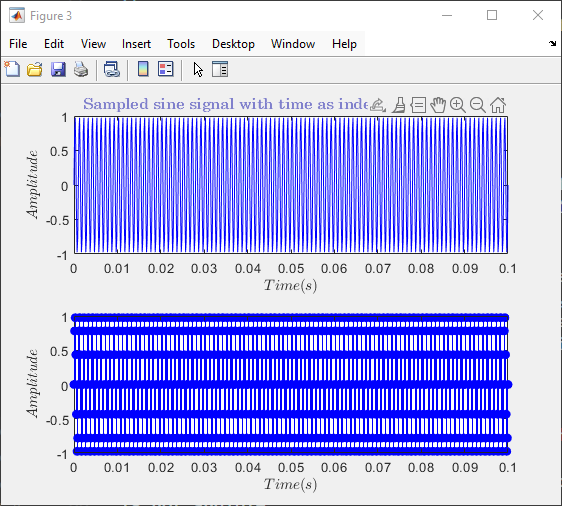
\includegraphics[width=0.3\textwidth]{fig 1f 7000.png}\hfill
% 	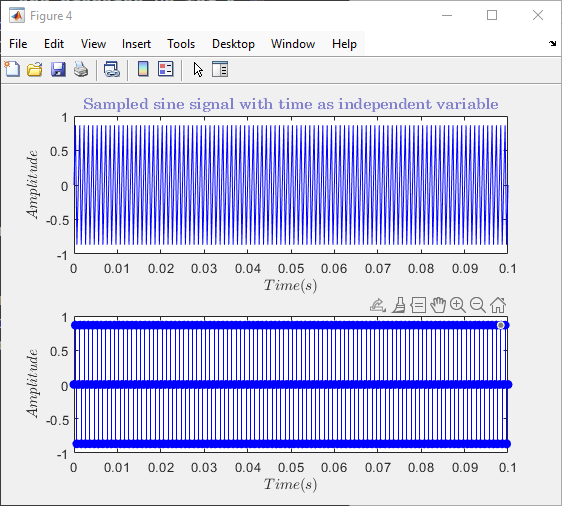
\includegraphics[width=0.3\textwidth]{fig 1f 3000.png}\hfill
% 	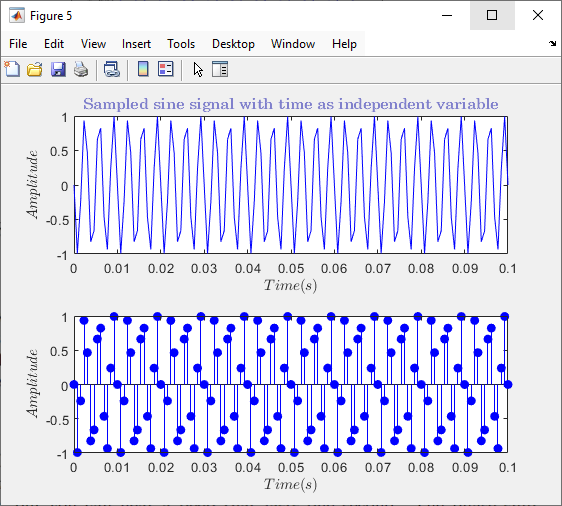
\includegraphics[width=0.3\textwidth]{fig 1f 1300.png}
% 	\caption{Sinusoidal with $f_s$ = 7 kHz, 3 kHz, and 1.3 kHz}
% 	\label{fig:fig3}
% \end{figure}
\begin{figure}[H]
	\centering
	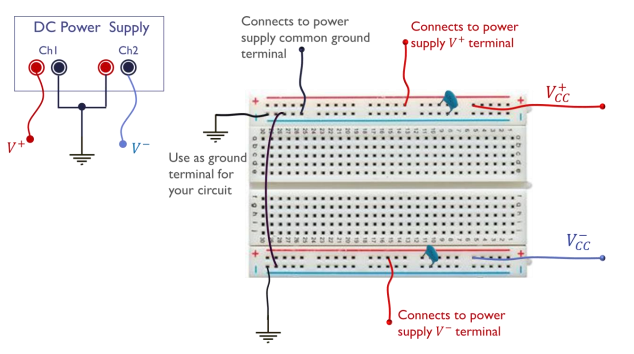
\includegraphics[width=0.5\textwidth]{powersuply connections.png}
	\caption{DC Power Supply Connections on Breadboard}
	\label{fig:fig1}
\end{figure}
An inverting op-amp circuit was constructed. First the DC power supply 
was connected to the breadboard as shown in Figure \ref{fig:fig1}. The 
two capacitors used had a capacitance of 10 $\mu$F.


\begin{figure}[H]
	\centering
	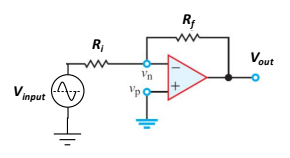
\includegraphics[width=0.25\textwidth]{inverting op-amp circuit.png}\hfill
	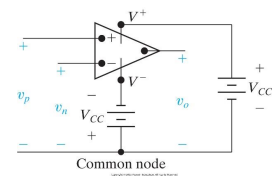
\includegraphics[width=0.25\textwidth]{dc power to op amp.png}\hfill
	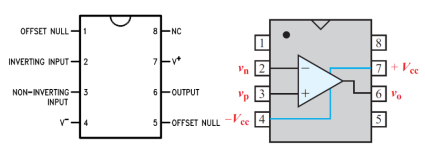
\includegraphics[width=0.4\textwidth]{op amp dip.png}
	\caption{Inverting Op-Amp Circuit}
	\label{fig:fig2}
\end{figure}

The inverting op-amp circuit was constructed as shown in Figure 
\ref{fig:fig2}. The gain of the circuit is chosen to be -10. The
equation for the gain of the inverting op-amp circuit is given by

\begin{equation*}
	G = -\frac{V_{out}}{V_{in}} = -\frac{R_f}{R_i}
\end{equation*}

Since we want a reistor value of 10 k$\Omega$ for $R_i$, we can choose
$R_f$ to be 100 k$\Omega$. The circuit was built on the breadboard in 
Figure \ref{fig:fig3}.

\begin{figure}[H]
	\centering
	\includegraphics[width=0.5\textwidth]{IMG_0364.png}
	\caption{Inverting Op-Amp Circuit on Breadboard}
	\label{fig:fig3}
\end{figure}

The actual values of $R_f$ and $R_i$ were measured to be 98.876 k$\Omega$
and 9.975 k$\Omega$ respectively. The circuit was then connected to 
a function generator which was set to produce a 1 kHz sine wave with an 
amplitude of 0.5 V peak-to-peak. An oscilloscope was connected to the
output of the op-amp circuit to measure the output voltage. The oscilloscope
was also connected directly to the function generator to measure the input.
The input voltange and output voltage were measured to be 1.11 V and 10.9 V,
respectively. The gain of the circuit was calculated to be -9.82, which is
close to the expected value of -10. The gain of the circuit is negative, because
the output sine wave has its phase shifted by $\pi$. The input sine wave
had the amplitude increased to 1.2V peak-to-peak. The output sine wave,
is measured to be 17.5 V with its peaks clipped. This is due to the 
op-amp reaching its maximum output voltage of $\pm 10$ V. If the voltage
cap was removed, then the amplitude would be 24 V.
\newline

The inverting op-amp circuit was then modified to include a DC offset. This
is called a summing inverting amplifier.

\begin{figure}[H]
	\centering
	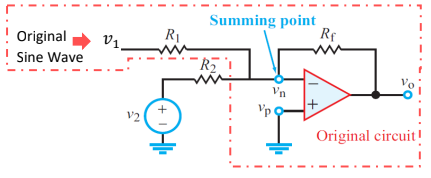
\includegraphics[width=0.5\textwidth]{summing inverting amplifier.png}
	\caption{Summing Inverting Amplifier}
	\label{fig:fig4}
\end{figure}

The circuit seen in Figure \ref{fig:fig4} was built on a breadboard. The
equation for the output voltage of the summing inverting amplifier is given
by the equation:

\begin{equation*}
	V_{out} = -\frac{R_f}{R_1}V_{1} - \frac{R_f}{R_2}V_{2}
\end{equation*}

The original circuits gain is $-\frac{R_f}{R_1} = -10$. Thus, the 
resistor value for $R_2$ can be calculated through this equation:

\begin{equation*}
	-\frac{R_f}{R_2}v_2 = -1 = -\frac{100 \; k \Omega}{R_2} \cdot 10 \; V \implies R_2 = 1 M \Omega
\end{equation*}

The circuit was built on a breadboard as shown in Figure \ref{fig:fig5}.
The actual values of the $R_2$ was measured to be $0.912 \; M \Omega$

\begin{figure}[H]
	\centering
	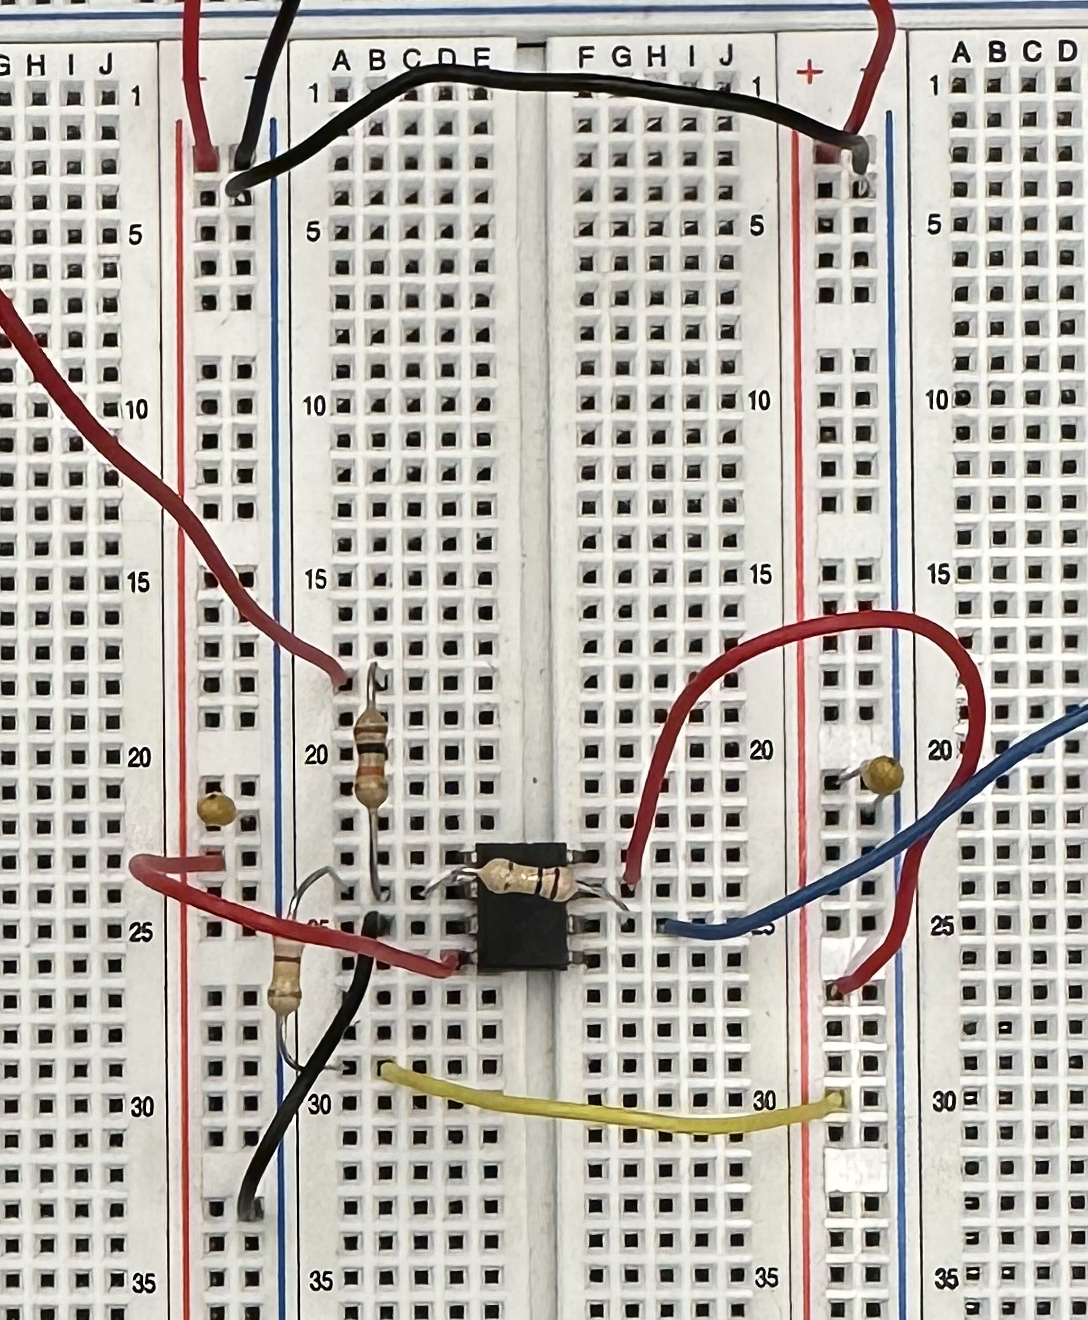
\includegraphics[width=0.3\textwidth]{IMG_0483.png}
	\caption{Summing Inverting Amplifier on Breadboard}
	\label{fig:fig5}
\end{figure}

The function generator was set to produce a 1 kHz sine wave with an 
amplitude of 0.5 V peak-to-peak. The DC power supply was set to 5 V.
In order to get the 10 V for $V_{out}$, $V_2$ is connected to $V_{cc}^+$.
The oscilloscope was connected to the output of the op-amp circuit to measure
the output voltage. The output voltage wasd measured to be 3.750 V peak-to-peak.
This is to be expected since the gain of the circuit is -10 and the DC offset
is -1 V. 


\section{Discussion and Conclusion}
In conclusion, this lab provided valuable hands-on experience with 
operational amplifiers, particularly inverting and summing inverting 
amplifier configurations. Through the construction and testing of these 
circuits, we observed how operational amplifiers manipulate input 
signals by controlling gain and polarity. The measured gain values 
were close to the theoretical predictions, demonstrating a solid 
understanding of circuit design and the influence of resistor values 
on gain.
\newline

In the inverting amplifier configuration, the expected gain of 
-10 was confirmed experimentally, with minor deviations due to 
component tolerances. The phase inversion characteristic of the 
inverting amplifier was clearly observed. The output clipping at high 
input signal amplitudes highlighted the importance of considering the 
op-amp's output voltage limits in practical circuit design.
\newline

The summing amplifier experiment further demonstrated the ability of 
op-amps to combine AC and DC signals. By introducing a DC offset, we 
successfully modified the output signal, reinforcing the utility of 
op-amps in applications requiring signal conditioning.
\newline

Overall, this lab established foundational knowledge of operational 
amplifier circuits, which will be crucial for more advanced analog 
electronics applications.


\section{References}
 [1] Dr. Iman Salama. “Lab 7 – Getting started with Operational Amplifier Circuits” Northeastern University. 25 October 2024.

\end{document}
